%%%%%%%%%%%%%%%%%%%%%%%%%%%%%%%%%%%%%%%%%%%%%%%%%
%%%%%%%%%%%% chap: Related Work%%%%%%%%%%%%%%%%%
%%%%%%%%%%%%%%%%%%%%%%%%%%%%%%%%%%%%%%%%%%%%%%%%%

\chapter{Related Work}\label{chapter:chap3}

\section{Similar Applications}\label{sect:similar applications}

\begin{wrapfigure}{r}{0.25\textwidth} 
    \centering
    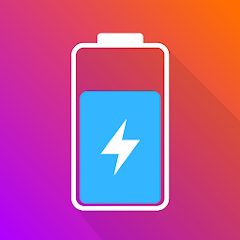
\includegraphics[width=0.25\textwidth]{app1.png}
\end{wrapfigure}

\textbf{1. Battery Saver}

\textbf{Developer}: Netroken

\textbf{Description}: Battery Saver lets the user monitor their battery level, using profiles that turn off battery-draining apps.

\textbf{Characteristics}:

• \textbf{Powerful Profiles}: The application automatically stops applications and services that consume the battery;

• \textbf{Set Battery Times}: The app can schedule profiles that can increase the battery life when the battery of the user drops to a set level;

• \textbf{Battery timeline}: The application lets you monitor your battery level in an orderly timeline;

• \textbf{Battery Availability}: The application shows how much time is left and what percentage of the battery is still valid;

• \textbf{Real-Time Notifications}: Notifications about battery life;

• \textbf{Save Battery Life}: The application offers the user the ability to configure settings for monitoring battery life.

\textbf{Data security}:

• This application may share these types of data with third parties;

• This application may collect these types of data (Location, in-app activity);

• Data is encrypted in transit;

• Data cannot be deleted.\newline

\begin{wrapfigure}{r}{0.25\textwidth} 
    \centering
    
\includegraphics[width=0.25\textwidth]{app2.png}
\end{wrapfigure}

\noindent 
\textbf{2. Phone Cleaner - Cache Clean}

\textbf{Developer}: Games Tree

\textbf{Description}: Phone cleaner is a cleaning app for an Android device and has the following characteristics: file cleaning capabilities, it can cool the CPU, a built-in application manager, and battery-saving functions.

\textbf{Characteristics}:

• \textbf{Cache Cleaner}: The app can clean apps or residual data, such as cache memory;

• \textbf{Storage Cleaner}: This function scans the phone for data to delete and free up space so it can increase the phone's performance;

• \textbf{CPU Cooling}: The app can cool the CPUs temperature and improve its performance;

• \textbf{Battery saving actions}: Another function of the app is the disabling of power-consuming apps;

• \textbf{Notification cleaning functions}: The last function of the app is its notification cleaning capabilities;

\textbf{Data security}:

• No data was collected;

• Data will be encrypted during transit;

• The user can request the data to be deleted;

• No data is shared with third parties.\newline

\begin{wrapfigure}{r}{0.25\textwidth} 
    \centering
    
\includegraphics[width=0.25\textwidth]{app3.png}
\end{wrapfigure}

\noindent 
\textbf{3. CCleaner – Phone Cleaner }

\textbf{Developer}: Piriform

\textbf{Description}: CCleaner helps you remove junk messages from your Android phone. This Android cleaning app clears your browser history, app cache, and clipboard contents. This Android device cleaner also helps to boot faster and provide better performance.

\textbf{Characteristics}:

• The app can clean cache memory, browser memory, and much more;

• Storage cleaning: The app can also analyze storage space and delete unwanted and residual data to boost performance;

• Application hibernation function, which allows the app to keep apps closed until opened manually;

• Ram boosting functions;

• Increases performance and battery life;

• Analyzes the impact of applications;

• Optimizes the storage of photos;

• Monitors the system.

\textbf{Data security}:

• The application may send different types of data to third parties;

• The application may collect the following types of data (Location, Personal Information);

• Data will be encrypted during the transmission period;

• The data can be deleted at request.\newline

\begin{wrapfigure}{r}{0.25\textwidth} 
    \centering
    
\includegraphics[width=0.25\textwidth]{app4.png}
\end{wrapfigure}

\noindent 
\textbf{4. Battery Guru: Battery Health }

\textbf{Developer}: Paget96

\textbf{Description}: Battery Guru displays information about battery usage, measures battery capacity (mAh), shows estimates and helps change charging habits with helpful tips to extend battery life and increase battery life.

\textbf{Characteristics}:

• Measures actual battery capacity (in mAh), dual battery configuration is also supported;

• The app can tell how much of the battery life the user has left;

• Advanced battery saving system;

• Support for dual battery configuration.

\textbf{Data security}:

• No data is shared with third parties;

• No data is collected.\newline

\begin{wrapfigure}{r}{0.25\textwidth} 
    \centering
    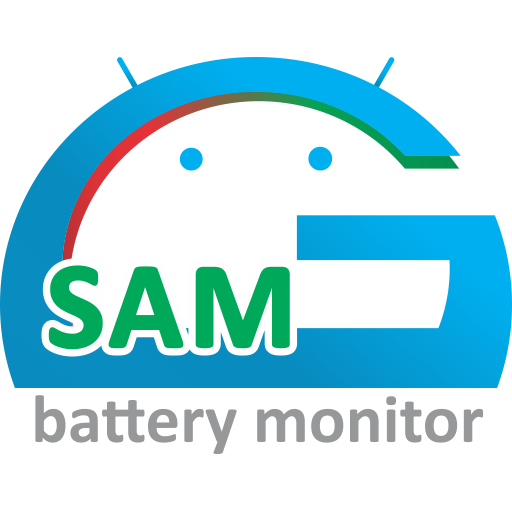
\includegraphics[width=0.25\textwidth]{app5.png}
\end{wrapfigure}

\noindent 
\textbf{5. GSam Battery Monitor }

\textbf{Developer}: GSam Labs

\textbf{Description}: GSam Battery Monitor is an application that aims to monitor the phone's battery and notify the user of the remaining battery time.

\textbf{Characteristics}:

• The app knows what apps consume the most battery;

• The app also shows the remaining battery life;

• The function to know how much the battery is being drained by different apps;

• The ability to list apps based on CPU usage, sensor usage, and so on;

• The user can set different time preferences to see how much battery was consumed in a set time period;

• The function to see the average lifespan of the battery;

• The app can also set alarms to keep the user informed of certain battery levels, temperature levels, and so on.

\textbf{Data security}:

• There is no public information.\newline

\begin{wrapfigure}{r}{0.25\textwidth} 
    \centering
    
\includegraphics[width=0.25\textwidth]{app6.png}
\end{wrapfigure}

\noindent 
\textbf{6. Droid Optimizer }

\textbf{Developer}: Ashampoo®

\textbf{Description}: Droid Optimizer is an application that aims to monitor the phone's battery, notify the user of the remaining battery time, optimize the phone and automatically perform cleaning tasks.

\textbf{Characteristics}:

• Performs cleaning tasks automatically;

• Find and delete unwanted files quickly and easily;

• Clears system and application cache;

• Automatically stops foreground and background applications;

• Accelerate, clean, and optimize;

• Saves energy and improves battery life;

• Disables WI-FI at predetermined times or every time the screen turns off;

• Manages applications;

• The app can expose apps that spy on their user and have critical permissions.

\textbf{Data security}:

• No data is shared with third parties;

• This application may collect these types of data: Location, application activity, and application information and performance;

• Data is encrypted in transit;

• Data cannot be deleted.


\section{Comparison}\label{sect:comparison}
    Each application presented has some specific characteristics, and although most of them have similar features, each one brings something different:

    1.	Droid Optimizer automatically turns off the user's mobile data and lets the user take a look at critical app permissions, exposing spy apps;
    
    2.	GSam sets customizable alarms for different states of charge, temperature, and battery status;

    3.	Battery Guru presents support for dual battery configuration;

    4.	CCleaner optimizes photo storage and presents the Task Killer functionality;

    5.	Phone Cleaner presents the Notification Cleaner functionality that deactivates and deletes unwanted notifications, if necessary;

    6.	Battery Saver has the ability to create profiles in order to optimize the phone's battery.


    The second, third, and last apps on this list focus only on saving battery life, while Phone Cleaner, CCleaner, and Droid Optimizer also focus on system cleaning and maintenance.
    
    From the point of view of data security, GSam does not provide information about this, Droid Optimizer, Battery Guru, and Phone Cleaner do not share data with third parties while CCleaner and Battery Saver share data, and from the point of view of data collection, Battery Guru and Phone Cleaner do not collect, while the rest of the applications collect data. 

    For the purpose of creating an application that is not a one-to-one copy of another, we need to look at these sorts of comparisons, to better understand what could be improved upon and added. As such, the following table, the one on the following page, offers a clear view of each functionality listed above and which app either has such an option or not.

    \begin{center}
    \begin{tabular}{ | >{\centering\arraybackslash}X m{3cm} | >{\centering\arraybackslash}X m{1.6cm} | >{\centering\arraybackslash}X m{1.6cm} | >{\centering\arraybackslash}X m{1.8cm} | >{\centering\arraybackslash}X m{1.7cm} | >{\centering\arraybackslash}X m{1.7cm} | >{\centering\arraybackslash}X m{2cm} | }
    \hline
        \textbf{Comparison} & \textbf{Battery Saver} & \textbf{Phone cleaner} & \textbf{CCleaner} & \textbf{Battery GURU} & \textbf{Gsam Monitor} & \textbf{Droid Optimizer} \\ \hline
        
        Battery Save & YES & YES & YES & YES & YES & YES \\ \hline
        
        Battery and phone state monitoring & YES & YES & YES & YES & YES & YES \\ \hline
        
        CPU cooling & NO & YES & NO & NO & NO & NO \\ \hline
        
        CPU Tracking & NO & YES & YES & NO & YES & YES \\ \hline
        
        Customizing the battery maintenance mode & YES & NO & NO & NO & YES & NO \\ \hline
        
        Deactivating WI-FI & NO & NO & NO & NO & NO & YES \\ \hline
        
        Automatic performance of cleaning tasks & NO & YES & YES & NO & NO & YES \\ \hline
        
        Managing critical permissions & NO & NO & NO & NO & NO & YES \\ \hline
        
        Automatic stopping of applications & NO & YES & YES & NO & NO & YES \\ \hline
        
        Battery life tracker & YES & NO & NO & YES & YES & NO \\ \hline
        
        Historical battery life averages & YES & NO & NO & NO & YES & NO \\ \hline
        
        Data collection & YES & NO & YES & NO & - & YES \\ \hline
        
        Double battery configuration support & NO & NO & NO & NO & YES & NO \\ \hline
        
        Optimizing the storage of photos & NO & NO & YES & NO & NO & NO \\ \hline
        
        Memory space recovery & NO & YES & YES & NO & NO & YES \\ \hline
        
        Notification cleaner & NO & YES & NO & NO & NO & NO \\ \hline
        
        Sharing with third parties & YES & NO & YES & NO & - & NO \\ \hline
        
        Encrypted data in transit & YES & YES & YES & - & - & YES \\ \hline
        
        Data may be deleted & NO & YES & YES & - & - & NO \\ \hline
        
    \end{tabular}
\end{center}
